\documentclass{csbeamer}

\usepackage{hyperref}
\usepackage{listings}
\usepackage{xcolor}
\usepackage{graphicx}

% Python code styling
\lstset{
    language=Python,
    basicstyle=\ttfamily\small,
    keywordstyle=\color{blue}\bfseries,
    stringstyle=\color{red},
    commentstyle=\color{green!50!black}\itshape,
    showstringspaces=false,
    breaklines=true,
    frame=single,
    numbers=left,
    numberstyle=\tiny\color{gray}
}

% Course information
\title{Introduction to Pictures and Pixels}
\course{CSCI 128: Introduction to Computer Science}
\courseshort{CSCI 128}
\term{Winter 2025}
\author{Dr. Jean-Alexis Delamer}

\begin{document}

\begin{frame}
\titlepage
\end{frame}

\begin{frame}{Welcome to Media Computation!}
    \begin{center}
        \Large Today we start working with pictures!
    \end{center}

    \vspace{1em}

    \textbf{Learning Objectives:}
    \begin{itemize}
        \item<1-> Understand how \textcolor{stfxblue}{digital images} are represented
        \item<2-> Learn about \textcolor{marigold}{pixels} and \textcolor{stfxblue}{RGB color model}
        \item<3-> Load and display images in Python
        \item<4-> Access pixel information
        \item<5-> Set up Pillow library for image manipulation
    \end{itemize}

    \vspace{1em}

    \begin{center}
        \onslide<6->{\textit{This is where programming becomes \textcolor{marigold}{\textbf{visual and fun!}}}}
    \end{center}
\end{frame}

\begin{frame}{Why Pictures?}
    \textbf{Working with images is:}
    \begin{itemize}
        \item<1-> More engaging than abstract problems
        \item<2-> Immediately \textcolor{marigold}{visual} - you see your results
        \item<3-> Practical - image processing is used everywhere
        \item<4-> A great way to learn programming concepts
    \end{itemize}

    \vspace{1em}

    \pause

    \textbf{Applications of image processing:}
    \begin{itemize}
        \item<6-> Social media filters (Instagram, Snapchat)
        \item<7-> Photo editing software (Photoshop, GIMP)
        \item<8-> Medical imaging (X-rays, MRIs)
        \item<9-> Computer vision (self-driving cars, face recognition)
        \item<10-> Special effects in movies
    \end{itemize}
\end{frame}

\begin{frame}{What is a Digital Image?}
    \begin{center}
        \Large A digital image is a \textcolor{marigold}{\textbf{grid of colored dots}}
    \end{center}

    \vspace{1em}

    \textbf{Key concepts:}
    \begin{itemize}
        \item<2-> \textcolor{marigold}{\textbf{Pixel:}} Short for "picture element" - one colored dot
        \item<3-> \textcolor{stfxblue}{\textbf{Resolution:}} Number of pixels (e.g., 1920×1080)
        \item<4-> \textcolor{stfxblue}{\textbf{Grid:}} Pixels arranged in rows and columns
    \end{itemize}

    \vspace{1em}

    \onslide<5->{Think of it like a mosaic or a cross-stitch pattern - from far away it looks like a continuous image, but up close you can see the individual pieces.}
\end{frame}

\begin{frame}{Pixels: The Building Blocks}
    \begin{center}
        \textbf{Every pixel has:}
    \end{center}

    \vspace{1em}

    \begin{enumerate}
        \item<1-> \textcolor{stfxblue}{\textbf{A position}} in the grid
            \begin{itemize}
                \item x-coordinate (column)
                \item y-coordinate (row)
                \item (0,0) is typically at top-left
            \end{itemize}

        \vspace{0.5em}

        \item<2-> \textcolor{marigold}{\textbf{A color}} represented by numbers
            \begin{itemize}
                \item We'll use the RGB color model
            \end{itemize}
    \end{enumerate}

    \vspace{1em}

    \begin{center}
        \onslide<3->{An 800×600 image has \textcolor{marigold}{\textbf{480,000 pixels!}}}
    \end{center}
\end{frame}

\begin{frame}{The RGB Color Model}
    \textcolor{marigold}{\textbf{RGB = Red, Green, Blue}}

    \vspace{1em}

    \textbf{How it works:}
    \begin{itemize}
        \item<1-> Every color is made by mixing \textcolor{red}{red}, \textcolor{green!50!black}{green}, and \textcolor{blue}{blue} light
        \item<2-> Each component has a value from \textcolor{stfxblue}{\textbf{0 to 255}}
        \item<3-> 0 = none of that color
        \item<4-> 255 = maximum intensity of that color
        \item<5-> $256 \times 256 \times 256 = \textcolor{marigold}{\textbf{16,777,216}}$ possible colors!
    \end{itemize}

    \vspace{1em}

    \pause

    \textbf{This is \textcolor{stfxblue}{additive} color mixing:}
    \begin{itemize}
        \item<7-> Like mixing colored lights (not paint!)
        \item<8-> Red + Green = Yellow
        \item<9-> Red + Blue = Magenta
        \item<10-> Green + Blue = Cyan
        \item<11-> Red + Green + Blue = White
    \end{itemize}
\end{frame}

\begin{frame}{RGB Examples}
    \begin{center}
        \begin{tabular}{|l|c|c|c|}
            \hline
            \textbf{Color} & \textbf{Red} & \textbf{Green} & \textbf{Blue} \\
            \hline
            Black & 0 & 0 & 0 \\
            \hline
            White & 255 & 255 & 255 \\
            \hline
            Pure Red & 255 & 0 & 0 \\
            \hline
            Pure Green & 0 & 255 & 0 \\
            \hline
            Pure Blue & 0 & 0 & 255 \\
            \hline
            Yellow & 255 & 255 & 0 \\
            \hline
            Magenta & 255 & 0 & 255 \\
            \hline
            Cyan & 0 & 255 & 255 \\
            \hline
            Gray & 128 & 128 & 128 \\
            \hline
        \end{tabular}
    \end{center}

    \vspace{1em}

    \textcolor{marigold}{\textbf{Notice:}} When R=G=B, you get shades of \textcolor{stfxblue}{gray!}
\end{frame}

\begin{frame}{Try It: RGB Colors}
    \begin{center}
        \Large \textbf{Activity Time!}
    \end{center}

    \vspace{1em}

    \textbf{What color do these RGB values make?}
    \begin{enumerate}
        \item (255, 165, 0)
        \item (128, 0, 128)
        \item (0, 128, 128)
        \item (255, 192, 203)
    \end{enumerate}

    \vspace{1em}

    \textbf{What RGB values would create:}
    \begin{enumerate}
        \item Dark red?
        \item Light blue?
        \item Brown (dark orange)?
    \end{enumerate}

    \vspace{1em}

    \textit{Hint: Higher values = brighter, lower = darker}
\end{frame}

\begin{frame}[fragile]{Python Libraries for Images}
    \textbf{We'll use Pillow (PIL - Python Imaging Library)}

    \vspace{1em}

    \textbf{Installation:}
    \begin{lstlisting}
# In your terminal/command prompt:
pip install Pillow
    \end{lstlisting}

    \vspace{1em}

    \textbf{Why Pillow?}
    \begin{itemize}
        \item<2-> \textcolor{marigold}{Easy to use}
        \item<3-> Well-documented
        \item<4-> Widely used in industry
        \item<5-> Supports many image formats (JPEG, PNG, GIF, etc.)
        \item<6-> Powerful image manipulation capabilities
    \end{itemize}
\end{frame}

\begin{frame}[fragile]{Loading an Image}
    \textbf{Basic steps to work with an image:}

    \begin{lstlisting}
from PIL import Image

# Load an image from a file
img = Image.open("beach.jpg")

# Display the image
img.show()
    \end{lstlisting}

    \vspace{1em}

    \pause

    \textbf{What happens:}
    \begin{itemize}
        \item<2-> \textcolor{stfxblue}{\texttt{Image.open()}} reads the image file
        \item<3-> Returns an Image object stored in \texttt{img}
        \item<4-> \textcolor{marigold}{\texttt{show()}} opens the image in your default viewer
    \end{itemize}

    \vspace{1em}

    \onslide<5->{\textcolor{red}{\textbf{Note:}} The image file must be in the same folder as your program (or provide full path)}
\end{frame}

\begin{frame}[fragile]{Getting Image Information}
    Once you've loaded an image, you can inspect it:

    \begin{lstlisting}
from PIL import Image

img = Image.open("beach.jpg")

# Get the dimensions
width, height = img.size
print(f"Width: {width}, Height: {height}")

# Get the color mode
print(f"Mode: {img.mode}")

# Get the format
print(f"Format: {img.format}")
    \end{lstlisting}

    \vspace{1em}

    \pause

    \textbf{Common modes:}
    \begin{itemize}
        \item<2-> \textcolor{marigold}{"RGB"} - Color image (3 channels)
        \item<3-> \textcolor{stfxblue}{"L"} - Grayscale (1 channel)
        \item<4-> "RGBA" - Color with transparency (4 channels)
    \end{itemize}
\end{frame}

\begin{frame}[fragile]{The Coordinate System}
    \textcolor{red}{\textbf{Important:}} Image coordinates start at \textcolor{marigold}{\textbf{(0, 0)}} in the \textcolor{stfxblue}{top-left corner!}

    \begin{center}
        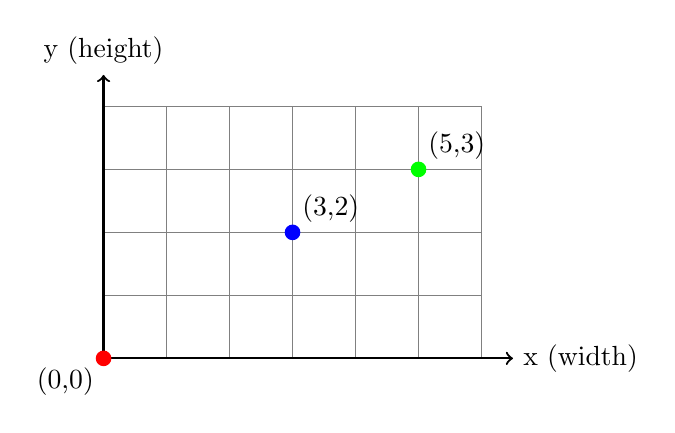
\begin{tikzpicture}[scale=0.8]
            % Draw grid
            \draw[step=1cm,gray,very thin] (0,0) grid (6,4);

            % Draw axes
            \draw[thick,->] (0,0) -- (6.5,0) node[right] {x (width)};
            \draw[thick,->] (0,0) -- (0,4.5) node[above] {y (height)};

            % Mark origin
            \node[circle,fill=red,inner sep=2pt] at (0,0) {};
            \node[below left] at (0,0) {(0,0)};

            % Mark some points
            \node[circle,fill=blue,inner sep=2pt] at (3,2) {};
            \node[above right] at (3,2) {(3,2)};

            \node[circle,fill=green,inner sep=2pt] at (5,3) {};
            \node[above right] at (5,3) {(5,3)};
        \end{tikzpicture}
    \end{center}

    \vspace{0.5em}

    \begin{itemize}
        \item<2-> \textcolor{stfxblue}{x} increases going \textcolor{marigold}{right}
        \item<3-> \textcolor{stfxblue}{y} increases going \textcolor{marigold}{down} (not up like in math!)
    \end{itemize}
\end{frame}

\begin{frame}[fragile]{Accessing Individual Pixels}
    \textbf{Get the color of a specific pixel:}

    \begin{lstlisting}
from PIL import Image

img = Image.open("beach.jpg")

# Get the color at position (100, 50)
pixel_color = img.getpixel((100, 50))
print(pixel_color)

# For RGB images, this returns a tuple: (R, G, B)
# Example output: (142, 198, 235)

# You can unpack it:
r, g, b = img.getpixel((100, 50))
print(f"Red: {r}, Green: {g}, Blue: {b}")
    \end{lstlisting}

    \vspace{1em}

    \pause

    \textcolor{marigold}{\textbf{Note:}} Coordinates are (x, y) - width first, then height!
\end{frame}

\begin{frame}[fragile]{Setting Pixel Colors}
    \textbf{You can also change pixel colors:}

    \begin{lstlisting}
from PIL import Image

img = Image.open("beach.jpg")

# Set pixel at (100, 50) to pure red
img.putpixel((100, 50), (255, 0, 0))

# Set another pixel to white
img.putpixel((101, 50), (255, 255, 255))

# Don't forget to save or show your changes!
img.show()
# or
img.save("modified_beach.jpg")
    \end{lstlisting}

    \vspace{1em}

    \pause

    \textcolor{red}{\textbf{Important:}} \texttt{putpixel()} modifies the image in memory, but doesn't save to disk automatically!
\end{frame}

\begin{frame}[fragile]{Try It: First Image Program}
    \begin{center}
        \Large \textbf{Activity Time!}
    \end{center}

    \vspace{1em}

    \textbf{Write a program that:}
    \begin{enumerate}
        \item Loads an image
        \item Prints its width and height
        \item Gets the color of the pixel at position (0, 0)
        \item Prints the RGB values
        \item Changes that pixel to bright green
        \item Displays the modified image
    \end{enumerate}

    \vspace{1em}

    \textcolor{marigold}{\textbf{Hint:}} Bright green is \textcolor{green!50!black}{\textbf{(0, 255, 0)}}

    \vspace{0.5em}

    \textit{You probably won't see the change - one \textcolor{stfxblue}{pixel} is tiny!}
\end{frame}

\begin{frame}[fragile]{Creating a New Image}
    \textbf{You can create blank images from scratch:}

    \begin{lstlisting}
from PIL import Image

# Create a 200x100 image with red background
img = Image.new("RGB", (200, 100), (255, 0, 0))
img.show()

# Create a 300x300 white image
img = Image.new("RGB", (300, 300), (255, 255, 255))

# Create a 400x400 black image
img = Image.new("RGB", (400, 400), (0, 0, 0))
    \end{lstlisting}

    \vspace{1em}

    \textbf{Parameters:}
    \begin{itemize}
        \item Mode: "RGB" for color images
        \item Size: (width, height)
        \item Color: (R, G, B) tuple for the fill color
    \end{itemize}
\end{frame}

\begin{frame}[fragile]{Drawing on Images}
    \textbf{Let's draw a simple pattern:}

    \begin{lstlisting}
from PIL import Image

# Create a 100x100 white image
img = Image.new("RGB", (100, 100), (255, 255, 255))

# Draw a red horizontal line across the middle
for x in range(100):
    img.putpixel((x, 50), (255, 0, 0))

# Draw a blue vertical line down the middle
for y in range(100):
    img.putpixel((50, y), (0, 0, 255))

img.show()
    \end{lstlisting}

    \vspace{1em}

    This creates a red cross pattern!
\end{frame}

\begin{frame}[fragile]{Loops with Pixels}
    \textbf{We can use loops to process many pixels:}

    \begin{lstlisting}
from PIL import Image

img = Image.new("RGB", (200, 100), (255, 255, 255))

# Make the top half blue
for x in range(200):
    for y in range(50):
        img.putpixel((x, y), (0, 0, 255))

# Make the bottom half red
for x in range(200):
    for y in range(50, 100):
        img.putpixel((x, y), (255, 0, 0))

img.show()
    \end{lstlisting}

    \vspace{1em}

    \pause

    \textcolor{marigold}{\textbf{Nested loops}} let us visit \textcolor{stfxblue}{\textbf{every pixel!}}
\end{frame}

\begin{frame}[fragile]{Efficient Pixel Access}
    \textbf{For processing many pixels, use load():}

    \begin{lstlisting}
from PIL import Image

img = Image.open("beach.jpg")
pixels = img.load()  # Load pixel data

width, height = img.size

# Now access pixels more efficiently
for x in range(width):
    for y in range(height):
        r, g, b = pixels[x, y]
        # Do something with the color
        # Modify if needed
        pixels[x, y] = (r, g, b)

img.show()
    \end{lstlisting}

    \vspace{1em}

    \texttt{load()} returns a pixel access object that's faster for repeated access
\end{frame}

\begin{frame}[fragile]{Try It: Create a Pattern}
    \begin{center}
        \Large \textbf{Activity Time!}
    \end{center}

    \vspace{1em}

    \textbf{Create a 200×200 image with:}
    \begin{enumerate}
        \item A red square in the top-left quadrant
        \item A green square in the top-right quadrant
        \item A blue square in the bottom-left quadrant
        \item A yellow square in the bottom-right quadrant
    \end{enumerate}

    \vspace{1em}

    \textbf{Hints:}
    \begin{itemize}
        \item Each quadrant is 100×100 pixels
        \item Top-left: x from 0-99, y from 0-99
        \item Remember: Yellow = (255, 255, 0)
    \end{itemize}
\end{frame}

\begin{frame}{Understanding Image File Formats}
    \textbf{Common formats:}

    \vspace{1em}

    \begin{itemize}
        \item \textbf{JPEG (.jpg, .jpeg)}
            \begin{itemize}
                \item Compressed, lossy format
                \item Good for photographs
                \item Smaller file sizes
            \end{itemize}

        \item \textbf{PNG (.png)}
            \begin{itemize}
                \item Compressed, lossless format
                \item Supports transparency
                \item Better for graphics with sharp edges
            \end{itemize}

        \item \textbf{GIF (.gif)}
            \begin{itemize}
                \item Limited to 256 colors
                \item Supports animation
            \end{itemize}

        \item \textbf{BMP (.bmp)}
            \begin{itemize}
                \item Uncompressed
                \item Large file sizes but no quality loss
            \end{itemize}
    \end{itemize}
\end{frame}

\begin{frame}[fragile]{Saving Images}
    \textbf{Save your modified images:}

    \begin{lstlisting}
from PIL import Image

img = Image.open("original.jpg")

# Modify the image somehow...
# ...

# Save in the same format
img.save("modified.jpg")

# Or save in a different format
img.save("modified.png")

# Specify quality for JPEG (1-100, default 75)
img.save("high_quality.jpg", quality=95)
    \end{lstlisting}

    \vspace{1em}

    \textbf{Tip:} The format is determined by the file extension!
\end{frame}

\begin{frame}[fragile]{Image Size Matters}
    \textbf{Consider image dimensions:}

    \vspace{1em}

    \begin{itemize}
        \item A 4000×3000 image has 12 million pixels!
        \item Processing every pixel can be slow
        \item Start with smaller images when testing
        \item You can resize images if needed
    \end{itemize}

    \vspace{1em}

    \begin{lstlisting}
from PIL import Image

img = Image.open("large_photo.jpg")
small_img = img.resize((400, 300))
small_img.save("small_photo.jpg")
    \end{lstlisting}

    \vspace{1em}

    \textbf{Tip:} Test your algorithms on small images first!
\end{frame}

\begin{frame}{What We Can Do With Pixels}
    Now that we understand pixels, we can:

    \vspace{1em}

    \begin{itemize}
        \item Change colors (filters, tints)
        \item Adjust brightness
        \item Convert to grayscale
        \item Flip and mirror images
        \item Detect edges
        \item Combine multiple images
        \item Create special effects
        \item And much more!
    \end{itemize}

    \vspace{1em}

    \begin{center}
        \textbf{All by manipulating individual pixel colors!}
    \end{center}
\end{frame}

\begin{frame}{Key Takeaways}
    \textbf{Today you learned:}
    \begin{itemize}
        \item Digital images are grids of colored pixels
        \item RGB color model uses red, green, and blue (0-255 each)
        \item How to load images with Pillow
        \item How to access and modify individual pixels
        \item Image coordinate system: (0,0) is top-left
        \item How to create new images from scratch
        \item How to save modified images
    \end{itemize}

    \vspace{1em}

    \begin{center}
        \textbf{You can now manipulate images programmatically!}
    \end{center}
\end{frame}

\begin{frame}{For Next Class}
    \textbf{Before next session:}
    \begin{itemize}
        \item Make sure Pillow is installed
        \item Find a few images to experiment with
        \item Try loading and inspecting different images
        \item Read Chapter 3 of the textbook
        \item Experiment with changing pixel colors
    \end{itemize}

    \vspace{1em}

    \textbf{Next session:}
    \begin{itemize}
        \item Processing all pixels in an image
        \item Creating filters (grayscale, negative, etc.)
        \item Image transformations
        \item Lab: Build your first image filter!
    \end{itemize}

    \vspace{1em}

    \begin{center}
        \textbf{Questions?}
    \end{center}
\end{frame}

\end{document}
